% This is a Basic Assignment Paper but with like Code and stuff allowed in it, there is also url, hyperlinks from contents included. 

\documentclass[11pt]{article}

% Preamble

\usepackage[margin=1in]{geometry}
\usepackage{amsfonts, amsmath, amssymb}
\usepackage{fancyhdr, float, graphicx}
\usepackage[utf8]{inputenc} % Required for inputting international characters
\usepackage[T1]{fontenc} % Output font encoding for international characters
\usepackage{fouriernc} % Use the New Century Schoolbook font
\usepackage[nottoc, notlot, notlof]{tocbibind}
\usepackage{listings}
\usepackage{xcolor}
\usepackage{blindtext}
\usepackage{hyperref}
\hypersetup{
    colorlinks=true,
    linkcolor=black,
    filecolor=magenta,      
    urlcolor=cyan,
    pdfpagemode=FullScreen,
    }

\definecolor{codegreen}{rgb}{0,0.6,0}
\definecolor{codegray}{rgb}{0.5,0.5,0.5}
\definecolor{codepurple}{rgb}{0.58,0,0.82}
\definecolor{backcolour}{rgb}{0.95,0.95,0.92}

\lstdefinestyle{mystyle}{
    backgroundcolor=\color{backcolour},   
    commentstyle=\color{codegreen},
    keywordstyle=\color{magenta},
    numberstyle=\tiny\color{codegray},
    stringstyle=\color{codepurple},
    basicstyle=\ttfamily\footnotesize,
    breakatwhitespace=false,         
    breaklines=true,                 
    captionpos=b,                    
    keepspaces=true,                 
    numbers=left,                    
    numbersep=5pt,                  
    showspaces=false,                
    showstringspaces=false,
    showtabs=false,                  
    tabsize=2
}

\lstset{style=mystyle}

% Header and Footer
\pagestyle{fancy}
\fancyhead{}
\fancyfoot{}
\fancyhead[L]{\textit{\Large{Information and Cycbersecurity - 2nd Year B. Tech}}}
%\fancyhead[R]{\textit{something}}
\fancyfoot[C]{\thepage}
\renewcommand{\footrulewidth}{1pt}



% Other Doc Editing
% \parindent 0ex
%\renewcommand{\baselinestretch}{1.5}

\begin{document}

\begin{titlepage}
    \centering

    %---------------------------NAMES-------------------------------

    \huge\textsc{
        MIT World Peace University
    }\\

    \vspace{0.75\baselineskip} % space after Uni Name

    \LARGE{
        Information and Cybersecurity\\
        Second Year B. Tech, Semester 1
    }

    \vfill % space after Sub Name

    %--------------------------TITLE-------------------------------

    \rule{\textwidth}{1.6pt}\vspace*{-\baselineskip}\vspace*{2pt}
    \rule{\textwidth}{0.6pt}
    \vspace{0.75\baselineskip} % Whitespace above the title



    \huge{\textsc{
            Implementation of Digital Signatures
        }} \\



    \vspace{0.5\baselineskip} % Whitespace below the title
    \rule{\textwidth}{0.6pt}\vspace*{-\baselineskip}\vspace*{2.8pt}
    \rule{\textwidth}{1.6pt}

    \vspace{1\baselineskip} % Whitespace after the title block

    %--------------------------SUBTITLE --------------------------	

    \LARGE\textsc{
        Lab Assignment 7
    } % Subtitle or further description
    \vfill

    %--------------------------AUTHOR-------------------------------

    Prepared By
    \vspace{0.5\baselineskip} % Whitespace before the editors

    \Large{
        Krishnaraj Thadesar \\
        Cyber Security and Forensics\\
        Batch A1, PA 20
    }


    \vspace{0.5\baselineskip} % Whitespace below the editor list
    \today

\end{titlepage}


\tableofcontents
\thispagestyle{empty}
\clearpage

\setcounter{page}{1}

\section{Aim}
Write a program using JAVA or Python or C++ to implement Digital signature using DSA

\section{Objectives}
To learn authentication technique for access control

\section{Theory}

\subsection{The Digital Signature Algorithm (DSA)}

The Digital Signature Algorithm (DSA) is a public key cryptographic algorithm that is used to create and verify digital signatures. It was developed by the US National Institute of Standards and Technology (NIST) and is based on the mathematical concept of modular exponentiation.

The DSA algorithm consists of three main components: key generation, signature generation, and signature verification.

\subsection{Algorithm}

\subsubsection{Key Generation:}

\begin{enumerate}
    \item Choose a prime number $p$ such that $p$ is 1024 bits or longer, and $p-1$ is divisible by a 160-bit prime number $q$.
    \item Choose an integer $g$ such that $1 < g < p$ and $g^{(p-1)/q} \bmod p \neq 1$.
    \item Choose a random integer $x$ such that $0 < x < q$.
    \item Compute $y = g^x \bmod p$.
    \item The public key is $(p, q, g, y)$, and the private key is $x$.
\end{enumerate}

\subsubsection{Signature Generation:}

\begin{enumerate}
    \item Choose a random integer $k$ such that $0 < k < q$.
    \item Compute $$r = (g^k \bmod p) \bmod q$$
    \item Compute $$s = k^{-1} (H(m) + xr) \bmod q$$ where $H(m)$ is the hash of the message $m$.
    \item The signature is $(r, s)$.
\end{enumerate}

\subsubsection{Signature Verification:}

\begin{enumerate}
    \item Verify that $0 < r < q$ and $0 < s < q$.
    \item Compute $w = s^{-1} \bmod q$.
    \item Compute $$u_1 = (H(m)w) \bmod q$$ and $$u_2 = (rw) \bmod q$$
    \item Compute $$v = ((g^{u_1} y^{u_2}) \bmod p) \bmod q$$
    \item If $v = r$, the signature is valid. Otherwise, it is invalid.
\end{enumerate}

\subsection{Example}

Here is an example of how the DSA algorithm works:

Suppose Alice wants to send a message to Bob and sign it using DSA. Alice and Bob have already generated their public and private keys.

\subsubsection{Signature Generation:}

\begin{enumerate}
    \item Alice chooses a random integer $k = 123$.
    \item Alice computes $$r = (g^k \bmod p) \bmod q = (2^{123} \bmod 467) \bmod 61 = 8$$
    \item Alice computes $$s = k^{-1} (H(m) + xr) \bmod q = 123^{-1} (H(m) + 22 \cdot 8) \bmod 61$$ where $H(m)$ is the hash of the message $m$.
    \item Alice sends the message and the signature $(r, s)$ to Bob.
\end{enumerate}

\subsubsection{Signature Verification:}

\begin{enumerate}
    \item Bob receives the message and the signature $(r, s)$ from Alice.
    \item Bob verifies that $0 < r < q$ and $0 < s < q$.
    \item Bob computes $$w = s^{-1} \bmod q = 123^{-1} \bmod 61 = 31$$
    \item Bob computes $$u_1 = (H(m)w) \bmod q$$ and $$u_2 = (rw) \bmod q$$where $H(m)$ is the hash of the message $m$.
    \item Bob computes $$v = ((g^{u_1} y^{u_2}) \bmod p) \bmod q = ((2^{39} \cdot 22^{43}) \bmod 467) \bmod 61 = 8$$
    \item Since $v = r$, the signature is valid, and Bob knows that the message was sent by Alice and has not been altered.
\end{enumerate}


\section{Platform}
\textbf{\textbf{Operating System}}: Arch Linux x86-64 \\
\textbf{\textbf{IDEs or Text Editors Used}}: Visual Studio Code\\
\textbf{\textbf{Compilers or Interpreters} }: Python 3.10.1\\

\section{Input and Output}

\begin{verbatim}

\end{verbatim}


\section{Code}
\lstinputlisting[language=Python, caption="SHA Integrity Check"]{../Programs/Assignment_7/digital_signatures.py}

\section{Conclusion}
Thus, we have seen how to implement digital signatures using DSA algorithm.
\clearpage

\section{FAQ}

\begin{enumerate}
    \item \textbf{What are various digital signatures algorithms?}\\
          \begin{enumerate}
              \item RSA (Rivest-Shamir-Adleman): The RSA algorithm is one of the most widely used public-key cryptographic algorithms. It is used for both encryption and digital signatures. RSA signatures are computed using the signer's private key and verified using their public key.

              \item DSA (Digital Signature Algorithm): The DSA algorithm is a public-key cryptographic algorithm used to create and verify digital signatures. It was developed by the US National Institute of Standards and Technology (NIST).

              \item ECDSA (Elliptic Curve Digital Signature Algorithm): The ECDSA algorithm is a variant of the DSA algorithm that uses elliptic curve cryptography instead of modular arithmetic. It is commonly used in mobile and IoT devices because it requires less computational power than other signature algorithms.

              \item EdDSA (Edwards-curve Digital Signature Algorithm): The EdDSA algorithm is another variant of the DSA algorithm that uses Edwards curves instead of elliptic curves. It is designed to be faster and more secure than other signature algorithms.
          \end{enumerate}

    \item \textbf{Draw the diagrams of digital signature generation and verification.}\\

          \begin{figure}[H]
              \centering
              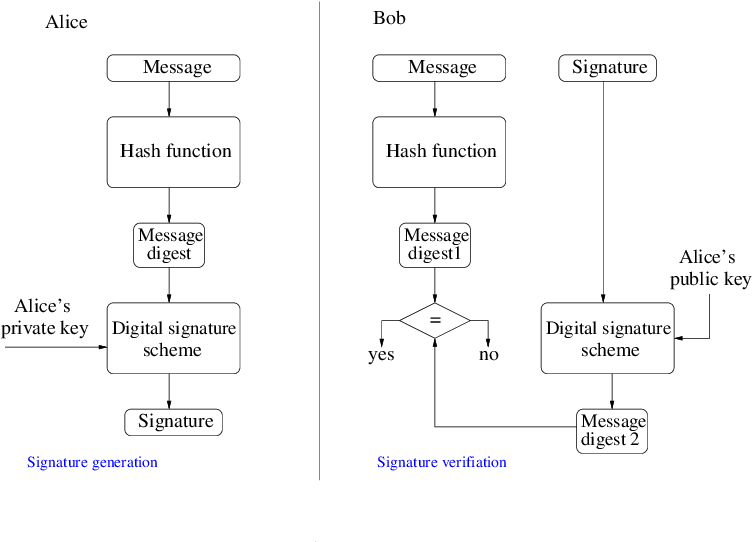
\includegraphics[width=.80\textwidth]{./Digital-signature-generation-and-verification.png}
              \caption{The General Process of Digital Signature Generation and Verification}
          \end{figure}

    \item \textbf{Which government agencies are involved to issue the digital signature? What is the validity of digital signature}\\


          \textbf{Government Agencies:}\\

          The government agencies involved in issuing digital signatures may vary depending on the country. In general, it is common for a government agency responsible for electronic signatures or digital certificates to issue digital signatures. \\

          For example, in the United States, the \textit{National Institute of Standards and Technology (NIST)} provides guidelines and standards for digital signatures and certificates.\\
    

          \textbf{Agencies in India}
          \begin{itemize}
              \item In India, digital signatures are issued by \textit{Certifying Authorities (CAs)} that are licensed by the Controller of Certifying Authorities (CCA). The CCA is a government agency under the Ministry of Electronics and Information Technology, responsible for the regulation and licensing of CAs in India. \\

              \item    The CCA is responsible for implementing the provisions of the Information Technology (IT) Act, 2000, which provides for the legal recognition of electronic records and digital signatures in India. The CCA issues licenses to CAs for issuing digital certificates, and also maintains a national repository of digital certificates that can be used to verify the authenticity of digital signatures.

              \item In addition to the CCA, the Ministry of Electronics and Information Technology and the Ministry of Law and Justice also play a role in the regulation and promotion of digital signatures and electronic transactions in India.

          \end{itemize}
          \textbf{Validity of Digital Signature:}\\

          The validity of a digital signature also varies depending on the country and the laws governing electronic signatures. In general, a digital signature is considered to be legally binding and valid if it meets certain criteria, such as:
          \begin{enumerate}

              \item The signature is created using a valid digital certificate issued by a trusted certification authority.
              \item The signer's private key is kept secure and not accessible to others.
              \item The signature was created at the time the document was signed and has not been altered since then.
              \item The certificate used to create the signature has not expired or been revoked.
              \item In most countries, digital signatures are considered to be as legally binding as traditional signatures.
              \item The validity of a digital signature can be verified by using the signer's public key to decrypt and verify the signature, and by checking the certificate used to create the signature to ensure that it is valid and has not been revoked.
          \end{enumerate}
\end{enumerate}

\end{document}